% !TEX root = ../Robotik.tex
\chapter{Lokalisation autonomer mobiler Robotersysteme}
\begin{description}
	\item[Lokalisation] Ermitteln der aktuellen Position des Roboters.
	\item[Pfadplanung oder Navigation] beantwortet die Fragen \textbf{Wie
		gelange ich dorthin?} Bewegungsplanung oder Pfadplanung bedeutet die
		Berechnung der Fahrroute und der daraus abgeleiteten Bahn vom aktuellen
		Punkt zum Zielpunkt. \\
		\textbf{Unterscheidung zwischen unbekannter und bekannter Umgebung}
	\item[Kartenerstellung, Mapping oder Umgebungsmodellierung] Die Auswertung
		der vom Roboter mittels Sensoren erfassten Daten der Umgebung mit dem
		Ziel, ein Umgebungsmodell zu erzeugen oder zu vervollständigen. \\
		$\Rightarrow$ Großes Problem
\end{description}

$\Rightarrow$ Selbstlokalisation und Kartenerstellung bedingen sich
gegenseitig.

\section{Varianten der Selbstlokalisierung}
\paragraph{Lokale Selbstlokalisierung (position tracking)}
\begin{itemize}
	\item Die Startposition des Roboters ist \textbf{ungefähr bekannt}.
	\item \textbf{Relative} Selbstlokalisierung
	\item Neuberechnung der Position mithilfe der Sensordaten bei Bewegung.
	\item Bezugspunkt ist der Startpunkt.
	\item \textbf{Methoden} sind Odometrie und Trägheitsnavigation
\end{itemize}

\paragraph{Globale Selbstlokalisierung}
\begin{itemize}
	\item Die Startposition ist unbekannt.
	\item \textbf{absolute Positionierung}
	\item Lokalisation durch Sensordaten und erkennen von \textbf{signifikanten}
		Umgebungsmerkmalen
	\item \textbf{Methode} ist Triangulation
\end{itemize}

\paragraph{Kidnapped Robot Problem}
\begin{enumerate}
	\item Die Position des Roboters ist anfangs bekannt
	\item Der Roboter wird willkürlich mit temporär deaktivierten Sensoren an eine beliebige andere Position versetzt, ohne darüber informiert zu werden.
	\item Auch dann muss das Verfahren robust die Position wiederfinden, zunächst muss der Roboter dies erkennen und sich dann relokalisieren
	\item Es muss eine erneute globale Lokalisierung durchgeführt werden
\end{enumerate}

\section{Relative Lokalisierung versus Absolute Lokalisierung}

\subsection*{Relative Lokalisierung}
\secsubtitle{
	Auch: \textbf{lokale}, \textbf{inkrementelle  Lokalisierung} oder 'tracking'.
}
Relativ zu einer Startpose wird sukzessiv die Änderung der Pose and disreten,
aufeinanderfolgenden Zeitpunkten ermittelt und integriert.

\subsection*{Absolute Lokalisierung}
\secsubtitle{
	Auch: \textbf{globale Lokalisierung}
}
Die Pose wird in Bezug auf ein externes Bezugssystem ermittelt, z.B. einer
Karte oder einem globalen Koordinatensystem

\paragraph{Ziel:} \hfill \\
Bestimme oder schätze die Position und Orientierung des Roboters in seiner
Umgebung basieren auf
\begin{itemize}
	\item der Eigenbewegung
	\item durch Messungen der relativen Position zu unterscheidbaren Objekten in
		der Umgebung in Roboterkoordinaten (Ultraschall, Laser, Kamera)
\end{itemize}
%BSP Chapter 3 Seite 4 / 28

\section{
	Transformation von Koordinatensystemen lokale $\leftrightarrow$ globale
}

{
\begin{wrapfigure}{r}{0.4\textwidth}
	\centering
	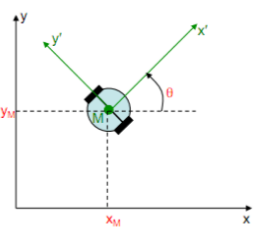
\includegraphics[width=0.39\textwidth]
		{Resources/PNG/transformationLocalGlobalBsp.png}
	\caption{}
\end{wrapfigure}

\paragraph{Kinematik} Die Kinematik ist die Lehre der Beschreibung von
Bewegungen von Punkten im Raum. Dabei werden die Größen Weg, Geschwindigkeit
und Beschleunigung betrachtet. Die Kinematik ist ein Teilgebiet der Mechanik.

\begin{description}
	\item[Kinematische Robotermodell] Kreisförmiger Roboter mit Zweiradantrieb
		und Bewegung in der Ebene.
	\item[Lokales Koordinatensystem] An den Roboter verbunden mit Ursprung in der
		Mitte der Antriebsachse. Die x-Achse zeight in Richtung des Roboterfront.
	\item[Roboterposition im globalen Koordinatensystem] \hfill \\
		Globale Koordinaten $M(x_M, y_M)$ und der Drehung von $x'$ im Bezug zu $x$
		als Winkel $\theta$. \\
		$\Rightarrow$ Pose $p$ mit $p = \colvec{x_M\\y_M\\\theta}$

\end{description}

}

\subsection*{Transformation von lokalen in globale Koordinaten}
\vspace{-0.6cm}
{
\begin{wrapfigure}{r}{0.4\textwidth}
	\centering
	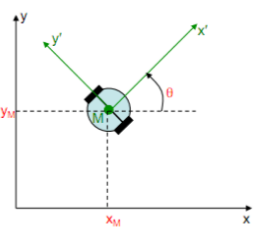
\includegraphics[width=0.25\textwidth]
		{Resources/PNG/transformationLocalGlobalBsp.png}
\end{wrapfigure}
\begin{align*}
	R_\alpha	&\mapsto\colvec{\sin\alpha&-\sin\alpha\\\sin\alpha & \cos\alpha} \\
	\vec{m} 	&= \colvec{x_M\\y_M} 																						 \\
	\vec{t}_g	&= R_\theta \cdot \colvec{x'\\y'} - \vec{m}
\end{align*}

}

\subsection*{Transformation von globalen in lokale Koordinaten}
\vspace{-0.6cm}
{
\begin{wrapfigure}{r}{0.4\textwidth}
	\centering
	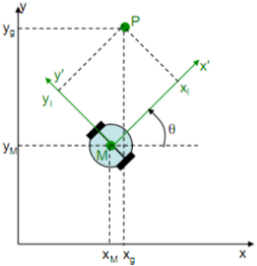
\includegraphics[width=0.25\textwidth]
		{Resources/PNG/transformationGlobalToLocal.png}
\end{wrapfigure}
\begin{align*}
	R_\alpha	&\mapsto\colvec{\sin\alpha&-\sin\alpha\\\sin\alpha & \cos\alpha} \\
	\vec{m} 	&= \colvec{x_M\\y_M} 																						 \\
	\vec{t}_l	&= R_{-\theta} \cdot \left(\colvec{x_g\\y_g} - \vec{m}\right)
\end{align*}

}

\section{Karten für statistische und dynamische Umgebungen}
Generell gilt: \textbf{Karten} sollen eine explizite Repräsentation des Raumes
sein.

Diese sind auf die Sensorik des Roboters zugeschnitten und nicht vorrangig für
den menschelichen Betrachter bestimmt.

\subsubsection*{Statische Umgebungen}
Basierend auf der Annahme, dass sich zwar der Zustand des Roboters innerhalb
der Umgebung, nicht jedoch die Umgebung selbst ändert.

$\Rightarrow$ Karte spiegelt die wirkliche Umgebung wieder.

\subsubsection*{Dynamische Umgebungen}
Objekte können ihre Lage oder ihren Zustand ändern. Dazu gehört das
verschwinden und auftauchen von bekannten oder unbekannten Objekten.

"Lernende" Karten sind ein fundamentales Problem in der mobilen Robotik

\subsection{Mapping Methoden}
Durch Koordinaten-Transformation kann zwischen den verschiedenen
Referenz-Frames beliebig ge\-wechselt werden.

\subsubsection{Weltzentriert}
Die Pose aller Objekte werden in der Umgebung in Bezug auf ein festes
Koordinatensystem repräsentiert.

Dies kann Indoor eine Zimmerecke sein und Outdoor ein globales
Koordinatensystem wie Längen- und Breitengrade, i.d.R. nutzen von
\textbf{WGRS}(World Geographic Reference System)

\subsubsection{Roboterzentriert}
Wird gebraucht um bspw. Kollisionen zu vermeiden. Diese nimmt als Bezugspunkt
den Roboter.

\subsection{Arten von Modellen}
Die wichtigste Form von Umgebungsmodellen für mobile Roboter sind
Umgebungskarten. Die folgende Ausführungen beziehen sich auf geeignet Karten
für \textbf{mobile, autonome Landfahrzeuge}

\begin{figure}[H]
	\begin{center}
		\includegraphics[scale=0.32]{Resources/PNG/MapTypes.PNG}
		\caption{Die verschiedenen Umgebungsmodelle}
		\label{fig:PNG/MapTypes.PNG}
	\end{center}
\end{figure}

\subsubsection{Arten von Umgebungsmodellen}
\begin{description}
	\item[Kontinuierliche metrische Karten] \hfill \\
	 	2D oder 3D bei denen jedes Objekt eine Koordinate erhält.
	\item[Diskrete  metrische Karten, Grid Maps] \hfill \\
		2D oder 3D bei der Raum in gleichmäßige oder ungleichmäßige Teile
		aufgeteilt wird. Ein Objekt wird mit einem dieser Teile assoziiert.
	\item[Hybrid Maps] \hfill \\
		z.B. Die Kontinuierliche metrische Anordnung von Grid Maps.
	\item[Topologische Modelle] \hfill \\
		Nur 2D bei der die Beziehung der Objekte zueinander im Vordergrund steht.
\end{description}

\subsection{Kontinuierliche Metrische Karten}
Metrische Lokalisierung beruht auf Ultraschall oder Laserscannern, bei der
eine exakte Beschreibung der Umgebung in 2D oder 3D möglich ist.

\textbf{Vorteil:} detailliertes Bild der Umgebung

\textbf{Nachteil:} große, unstrukturierte Datenmengen erschweren die
Pfadplanung

\subsection{Grid Maps - Rasterkarten}
{
\begin{wrapfigure}{r}{0.4\textwidth}
	\includegraphics[width=0.4\textwidth]{Resources/PNG/QuadTrees.png}
	\caption{oben: gleichmäßiges Gitter, unten: adaptives Gitter}
\end{wrapfigure}

Die Umwelt wird in gleichmäßiges Raster oder Grid zerlegt. Wobei für jede Zelle
mitgeführt wird ob sie belegt ist oder nicht. Dabei können je nach Modell
unterschiedliche Werte verwendet werden.
\begin{itemize}
	\item frei und belegt
	\item frei, belegt und Mischbelegung
	\item Belegungswahrscheinlichkeit
\end{itemize}
Notwendige Informationen sind z.B.:
\begin{itemize}
	\item x, y als Koordinaten (Zeile, Spalte) einer Zelle
	\item Sensordaten des Roboters
	\item Belegungswert
\end{itemize}
Dabei sind die Zellen unabhängig voneinander. Je höher die Messgenauigkeit der
Sensoren ist, desto kleiner können die Rasterelemente gewählt werden.

}

\subsubsection{Gleichmäßige Gitterstruktur vs. Adaptiver Gitterstruktur}
Für eine kompakte Notation können Grid Maps adaptive Unterteilt werden und im
2-dimensionalen Raum mit Quadtrees im 3-dimensionalen mit Octtrees gespeichert
werden.

\subsection{Adaptive Unterteilung}
\begin{enumerate}
	\item Ausgangszustand: Rechteck mit Hindernissen
	\item Fläche wird unterteilt in 4 Rechtecke gleicher Größe
	\item Jedes Rechteck wird rekursiv wieder in 4 Rechtecke unterteilt
		$\Rightarrow$ Quadtree
	\item Attributierung der Knoten:
		\begin{description}
			\item[Frei:] Rechteck enthält keinen Teil eines Hindernisses
			\item[Belegt:] Rechteck ist vollständig von Hindernis belegt
			\item[Gemischt:] Rechteck enhält nur Teile eines Hindernisses
		\end{description}
	\item Nur gemischte Knoten werden weiter unterteilt
\end{enumerate}
\subsubsection{Vorteile}
Schnell und leicht feststellbar, ob Punkt in einem Hindernis liegt

\subsubsection{Nachteile}
\begin{itemize}
	\item Konturen der Objekte und der Freiraum zwischen ihnen wird unpräzise repräsentiert
	\item Um die Datenfülle zu reduzieren, wird das Raster zu grob gewählt und dadurch ein möglicher Weg durch Mischpixel versperrt
\end{itemize}

{
\begin{wrapfigure}{r}{0.4\textwidth}
	\vspace{-1cm}
	\includegraphics[width=0.4\textwidth]{Resources/PNG/Trajektorie}
\end{wrapfigure}

\subsubsection{Weiterer Verwendungszweck}
Neben der reinen Lokalisierung können die Karten auch dazu verwendet werden
eine Fahrspur (Trakektorie) zu berechnen.

}

\subsubsection{Weitere Beispiele für Umgebungskarten}
\begin{itemize}
	\item Laserscan Karten
	\item Bildbasierte Karten
\end{itemize}

\subsection{Topologische Karten}
Bedingt geeignet zur Lokalisation, Haupteinsatzgebiet ist die Pfadplanung.
\begin{figure}[H]
	\begin{center}
		\includegraphics[scale=0.42]{Resources/PNG/TopologischeKarte.PNG}
		\caption{}
		\label{fig:PNG/TopologischeKarte.PNG}
	\end{center}
\end{figure}
\begin{itemize}
	\item Modelle bilden einen \textbf{Graphen}
	\item \textbf{Knoten} entsprechen Orten oder Bereichen der Umgebung
	\item Beziehungen zwischen den Orten werden durch \textbf{Kanten} modelliert.
	\item Zwei Knoten sind durch eine Kante verbunden, wenn sie unmittelbar
		voneinander erreichbar sind.
	\item \textbf{Gewichte}: Maß für die Länge der Wege
	\item Ist die Länge der jeweiligen Wegstücke bekannt, lässt sich der
		kürzeste Weg finden.
\end{itemize}

\paragraph{Vorteile}
\begin{itemize}
	\item Kompaktheit
	\item Gute Skalierbarkeit für welträumige Umgebungen.
	\item Es gibt viele schnelle Algorithemn auf Graphen, die gut zur
		Pfadplanung eingesetzt werden können
\end{itemize}

\paragraph{Nachteil} Relevante Umgebungsmerkmale werden verdeckt. Landmarken
werden schwerer erkannt.

\subsection{Hybrid Maps}
\begin{itemize}
	\item Kombinieren metrische und topologische Ansätze
	\item Ermöglichen Lokalisation und Kantenerstellung mit hoher Präzision
	\item Erhalten die Kompaktheit der topologischen Ansätze
\end{itemize}

\paragraph{Abstraktions-basierter Ansatz}
\begin{itemize}
	\item Basis: konstruieren einer metrischen Karte der Umgebung
	\item $\Rightarrow$ aufbau einer kompakten topologischen Repräsentation
	\item \textbf{Vorteil} Effizient Planung eines Pfads zu einem gegebenen Ziel
		aufgrund der Abstraktion.
	\item Die zugrunde liegende metrische Karte wird für Relokalisation und
		Hindernisvermeidung benötigt.
\end{itemize}

\section{Passive und Aktive Selbstlokalisierung}
\subsubsection*{Passive Verfahren}
\begin{itemize}
	\item bestimmen oder schätzen die Roboterposition mittels aktueller
		Sensorinformationen
	\item beeinflussen \textbf{nicht} die Bewegung und Orientierung des Roboters
	\item Lokalisierungsmodul beobachtet nur die Roboteroperationen
	\item Roboter bewegt sich zufällig hin und her bzw. führt die zu erledigende
		Aufgabe durch
\end{itemize}

\subsubsection*{Aktive Verfahren}
\begin{itemize}
	\item besitzen vollständige oder teilweise Kontrolle über die Bewegungen des
		Roboter und Ausrichtung der Sensoren
	\item fährt gezielt bestimmte Orte an um Mehrdeutigkeiten zwischen mehreren
		Orten aufzulösen
\end{itemize}

\section{Landmarken}
\subsubsection*{Definition}
Als Landmarken werden \textbf{eindeutig identifizierbare Charakteristiken der
Umwelt} bezeichnet, die von entsprechenden Sensoren erkannt werden können.

\paragraph{Landmarke}
\begin{itemize}
	\item ihre Position im Weltmodell ist bekannt
	\item sichtbar von unterschiedlichen Positionen aus
	\item erkennbar unter verschiedenen Belichtungen und Blickwinkeln
	\item relative Position bestimmbar
	\item stationär, oder dem Navigationsmechanismus musss die Bewegung bekannt
		sein
\end{itemize}

\paragraph{Vorteil} Navigation erfolgt mit der Umwelt selbst und nicht mittels
erechneter Daten

\subsubsection*{Natürliche Landmarken}
\begin{itemize}
	\item Werden nicht zum Zweck der Positionsbestimmung aufgestellt, können
		aber dafür verwendet werden
	\item Grundsätzlich Passiv
\end{itemize}

\subsubsection*{Künstliche Landmarken}
Markante Objekte, eigens zum Zwech der Positionsbestimmung in der Umgebung
installiert.
